\documentclass[lettersize,journal]{IEEEtran}
\usepackage{amsmath,amsfonts}
\usepackage{algorithmic}
\usepackage{algorithm}
\usepackage{algpseudocode}
\usepackage{array}
\usepackage[caption=false,font=normalsize,labelfont=sf,textfont=sf]{subfig}
\usepackage{textcomp}
\usepackage{stfloats}
\usepackage{url}
\usepackage{verbatim}
\usepackage{graphicx}
\usepackage{cite}
\usepackage{natbib}
\usepackage{amsmath}
\hyphenation{op-tical net-works semi-conduc-tor IEEE-Xplore}
\usepackage[colorlinks=true, linkcolor=black, citecolor=black, urlcolor=black]{hyperref}
% \usepackage[style=numeric, sorting=nyt]{biblatex}
% \addbibresource{references.bib}
% updated with editorial comments 8/9/2021

\begin{document}

\title{Reinforcement Learning Project 1 Report\\ Desperately Seeking Sutton - TD(\lambda)}

\author{Xingyan Liu (202264690069@mail.scut.edu.cn), Shiyi Wang (202230055267@mail.scut.edu.cn) \\Wolin Liang (202264690304@mail.scut.edu.cn), Haoming Jia (202264690267@mail.scut.edu.cn) 
\thanks{Liu Xingyan: Responsible for code programming, results collation and analysis.Wang Shiyi: Focuses on literature research and problem modeling, specifically defining the problem environment.Liang Wolin: Handles the introduction of related work and paper analysis.Jia Haoming: Analyzes the experimental results and their significance.}% <-this % stops a space
\thanks{Manuscript revised September 30, 2024.}}

% The paper headers
\markboth{Group 1 for Reinforcement Learning, Fall~2024}%
{Shell \MakeLowercase{\textit{et al.}}: A Sample Article Using IEEEtran.cls for IEEE Journals}


\maketitle

\begin{abstract}
This project report discuss the fundamentals of Temporal Difference (TD) Learning and provides details of steps in reproducing experiment results in Sutton’s paper “Learning to Predict by the Methods of Temporal Differences”
 using the bounded random-walk process.
\end{abstract}

\section{Introduction}
% \IEEEPARstart{T}{his} file is intended to 
% This file is intended to introduce a novel method to calculate 123456

% Para2

% 首先讲一下强化学习和梯度下降的发展历史。(before 1988)
% 然后简要介绍一下时序微分的思想
% 最后介绍一下本文的结构,intro结束。

% 强化学习的目的在于不通过显示编程的方式,让agent在于环境交互的过程中学习到最优化完成任务的策略。最早的之一关于强化学习的讨论是Steps Toward Artificial Intelligence(Minsky).此后强化学习的理论不断发展,并在机器人学(文献)、游戏理论(文献)中有广泛的应用。此外,随着深度神经网络的发展,深度强化学习(找一下文献)极大的赋能了强化学习领域,使其具备更强大的学习能力。深度神经网络的理论基础是梯度下降(找一下文献),这也同时是本篇论文所讨论的重点。梯度下降既是神经网络学习的原理,同样也是时序微分(Sutton论文)的原理。

Reinforcement learning aims to enable an agent to learn the optimal strategy for completing tasks through interaction with the environment, without explicit programming. One of the earliest discussions on reinforcement learning can be traced back to Minsky's \textit{Steps Toward Artificial Intelligence}. Since then, the theory of reinforcement learning has continuously developed and found widespread applications in robotics \cite{Kober2013}, and game theory \cite{Fudenberg1998}.

With the advancement of deep neural networks, deep reinforcement learning \citep{Mnih2015} has significantly empowered the field, providing it with more robust learning capabilities. The theoretical foundation of deep neural networks is gradient descent \cite{Rumelhart1986}, which is also a focus of this paper. Gradient descent is not only the principle behind neural network learning but also the basis of temporal difference learning \cite{Sutton1988}.

A cornerstone of this field is the concept of temporal difference (TD) learning, introduced by Richard S. Sutton in his seminal 1988 paper, "Learning to Predict by the Methods of Temporal Differences." This paper laid the groundwork for many of the advancements seen in reinforcement learning today.

Temporal difference learning represents a novel approach to prediction problems, where the objective is to forecast future outcomes based on current and historical data. Unlike traditional supervised learning, which relies on fixed target values, TD learning dynamically updates predictions by leveraging the discrepancies between successive predictions—hence the term "temporal difference". This innovative method allows for more flexible and adaptive learning processes, which are particularly beneficial in environments where outcomes are uncertain and evolve over time.

The implications of Sutton's temporal difference learning extend far beyond the initial prediction tasks it was designed to address. It has become a fundamental building block for more advanced reinforcement learning algorithms, such as Q-learning\cite{Watkins1989} and SARSA\cite{Rummery1994}, which have been applied successfully in a wide range of domains, from game playing to robotics. By enabling agents to learn effectively from their interactions with the environment, TD learning has significantly advanced the capabilities of artificial intelligence systems.

In this paper, we explore the principles of temporal difference learning as introduced by Sutton, examining its theoretical underpinnings, practical applications, and impact on the field of reinforcement learning. Through this exploration, we aim to highlight the enduring relevance and potential of TD learning in developing intelligent systems capable of adapting to complex and changing environments.

\section{Temporal Difference Learning Methods}

Temporal Difference (TD) learning is a core technique in \textbf{reinforcement learning}, primarily used to solve prediction and decision-making problems. It updates models by comparing the \textbf{differences between consecutive predictions over time}, unlike traditional supervised learning methods. This allows TD to perform incremental learning even \textbf{without explicit labels or outcomes}.

\subsection{Difference between TD and Traditional Supervised Learning}
\begin{itemize}
    \item \textbf{Supervised learning} relies on explicit labels, adjusting the model by comparing the prediction with the actual outcome. It requires a complete dataset, where each input has a corresponding output.\\
    For simplicity, Sutton suggests a special case where the prediction at time \( t \) is a function of the current state \( x_t \) and some learnable weights \( w \): \( P(x_t, w) \), where \( w(i) \) and \( x_t(i) \) are the \(i\)th dimension of \( w \) and \( x_t \):
\[
P_t = w^T x_t = \sum_i w(i) x_t(i)
\]

The weights update/learning procedure is derived as below where \( \alpha \) is the learning rate:
\[
\Delta w_t = \alpha (z - P_t) \nabla_w P_t = \alpha (z - w^T x_t) x_t
\]

For supervised learning schema, vector weights \( w \) is only updated after a complete observation-outcome sequence:
\[
w_{\text{new}} = w_{\text{old}} + \sum_{t=1}^{m} \Delta w_t
\]

    \item \textbf{TD learning} is different in that it does not require the final result immediately. Instead, it updates based on the \textbf{difference between consecutive predictions over time}. For instance, in a game, TD can estimate the future return of the current state without waiting for the game to end. This makes TD \textbf{more efficient in dynamic systems}.
\end{itemize}

\subsection{Basic Concept of TD Learning}
The core idea of TD learning is to update the value of a state by comparing the predictions at two consecutive time steps. The update rule is:
\[w_{new}=w_{old}+\sum_{t=1}^m\alpha(P_{t+1}-P_t)\sum_{k=1}^t\nabla_wP_k\]

\[
\Delta w_t = \alpha (P_{t+1} - P_t) \sum_{k=1}^{t} \lambda^{t-k} \nabla_w P_k
\]
where:
\begin{itemize}
    \item \(P_t\) and \(P_{t+1}\) are the predicted values at times \(t\) and \(t+1\),
    \item \(\alpha\) is the learning rate,
    \item \(\lambda\) is the trace-decay parameter,
    \item \(\nabla_w P_k\) is the gradient of the predicted value with respect to the weights at time \(k\).
\end{itemize}

\subsection{Introduction to TD(\!$\lambda$) Method}
TD(\!$\lambda$) is an extension of the basic TD method that introduces \textbf{eligibility traces} and a \textbf{decay factor \!$\lambda$}, enabling the method to update the value of not just the current state, but also the previous states based on their eligibility.

The eligibility traces can be incrementally computed using the following formula:
\[
e_{t+1} = \sum_{k=1}^{t+1} \lambda^{t+1-k} \nabla_w P_k = \nabla_w P_{t+1} + \lambda e_t
\]
This mechanism allows for more efficient computation of weight updates while maintaining eligibility traces over time.



para3

\section{Experiment \& Results}
In this section, we provide a comprehensive technical account of the reproduction of Figure 3-5 from Sutton's seminal work. Initially, the theoretical or optimal predicted values for non-terminal states in the random walk problem are derived using the methodology outlined in the paper. Two key experiments are then conducted: the first experiment focuses on repeated training sequence presentations across varying \(\lambda\) values, while the second experiment investigates the effect of single-sequence presentations under unbiased initialization, evaluating various \(\lambda\)-learning rate pairings.

\subsection{Theoretical Values of Weights in Random-Walk}

Let \(\mathbf{Q}\) represent the transition probability matrix between non-terminal states, with \(Q_{ij}\) as the probability of transitioning from state \(i\) to state \(j\), and \(\mathbf{h}\) as the transition probability vector to the terminal state \(G\). The expected outcome \(z\) for starting in state \(i\) is:

\[
E[z \mid i] = \left[ \sum_{k=0}^{\infty} \mathbf{Q}^k \mathbf{h} \right]_i = \left[ (\mathbf{I} - \mathbf{Q})^{-1} \mathbf{h} \right]_i
\]

Thus, the theoretical weights for the non-terminal states \(B, C, D, E, F\) are:

\[
\mathbf{w} = (\mathbf{I} - \mathbf{Q})^{-1} \mathbf{h}
\]

For the random-walk, \(\mathbf{Q}\) and \(\mathbf{h}\) are defined as:

\[
\mathbf{Q} = \begin{pmatrix}
0 & 0.5 & 0 & 0 & 0 \\
0.5 & 0 & 0.5 & 0 & 0 \\
0 & 0.5 & 0 & 0.5 & 0 \\
0 & 0 & 0.5 & 0 & 0.5 \\
0 & 0 & 0 & 0.5 & 0
\end{pmatrix}, \quad
\mathbf{h} = \begin{pmatrix}
0 \\
0 \\
0 \\
0 \\
0.5
\end{pmatrix}
\]

The resulting theoretical weight vector is:

\[
\mathbf{w} = \begin{pmatrix}
\frac{1}{6} \\
\frac{1}{3} \\
\frac{1}{2} \\
\frac{2}{3} \\
\frac{5}{6}
\end{pmatrix}
\]

\begin{algorithm}[H]
\caption{TD($\lambda$) with Repeated Presentations}\label{alg:td_lambda}
\begin{algorithmic}
    \STATE 
    \STATE \textsc{Input:} Python lists of $\lambda$ values
    \STATE \textsc{Output:} Dictionary storing the mean RMSE for each $\lambda$: \texttt{rmse\_dict}
    \STATE 
    \STATE \textsc{Initialize} list of $\lambda$, learning rate $\alpha$, stopping criteria $\epsilon$
    \FOR{each $\lambda$}
        \FOR{each training set}
            \STATE \textsc{Initialize} weights $w$
            \WHILE{changes in $w < \epsilon$}
                \FOR{each training sequence}
                    \STATE \textsc{Initialize} error \texttt{err}
                    \FOR{each state}
                        \STATE \textsc{Calculate} \texttt{err} and $\Delta w$
                    \ENDFOR
                    \STATE \textsc{Accumulate} $\Delta w$ across sequences
                \ENDFOR
                \STATE \textsc{Update} $w$ using accumulated $\Delta w$
            \ENDWHILE
            \STATE \textsc{Calculate} RMSE for the current training set
        \ENDFOR
        \STATE \textsc{Calculate} mean RMSE across all training sets
    \ENDFOR
\end{algorithmic}
\label{alg:td_lambda}
\end{algorithm}

\subsection{Repeated Presentations Paradigm}

100 randomly generated training sets, each containing 10 bounded random-walk sequences, were prepared using the methods outlined in Section II of this report.

In the repeated presentations paradigm, for a given $\lambda$ value, the learner is exposed to the 10 random-walk sequences in a training set multiple times until convergence. The weight adjustments, $\Delta w$, are accumulated across the 10 sequences, and weight updates occur only after a full epoch. This process is repeated for all 100 training sets, and the average root mean squared error (RMSE) is computed between the learned weights and the ideal weights of the non-terminal states: $X_B$, $X_C$, $X_D$, $X_E$, $X_F$.

\begin{figure}[ht]
    \centering
    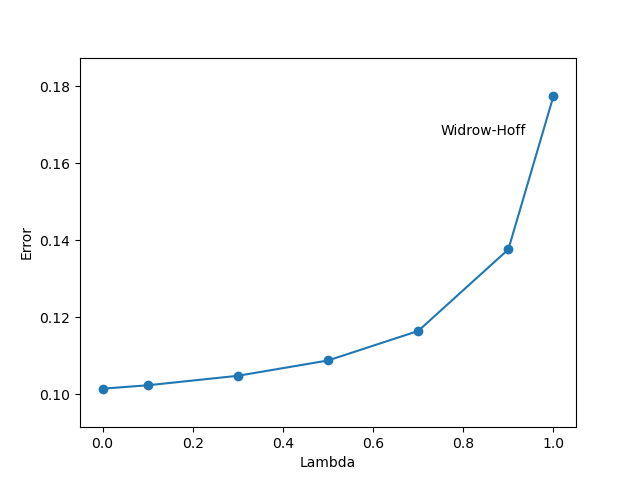
\includegraphics[width=0.8\linewidth]{figure3.png} 
    \caption{Average errors on the random-walk with repeated presentations.}
    \label{fig:avg_errors_random_walk}
\end{figure}

Figure 1 illustrates the average error between the learned weights $w$ and the ideal weights $\left[\frac{1}{6}, \frac{1}{3}, \frac{1}{2}, \frac{2}{3}, \frac{5}{6}\right]^T$ for various values of $\lambda$. The results show that TD(1) (Widrow-Hoff) yields the highest error compared to other values of $\lambda$. This could be attributed to TD(1)'s tendency to minimize the error between predictions and outcomes within the training set, without necessarily improving future predictions. In contrast, TD(0) achieves the lowest mean error, as it prioritizes the most recent state, aligning with the maximum likelihood estimation (MLE) for a Markov process.

The reproduced results closely match those in Figure 3 of Sutton’s paper, though the exact error values are somewhat lower. This discrepancy could be due to differences in the randomly generated training sets, as well as variations in initial weight settings and the learning rate $\alpha$, which were not explicitly defined in Sutton’s original experiment. In this reproduction, a learning rate of $\alpha = 0.01$ and unbiased weight initialization were used to ensure convergence in the TD learning process.

\subsection{Single Presentation Paradigm}

The same 100 randomly generated training sets used in the previous experiment were utilized in this paradigm. The weights were initialized with an unbiased value of 0.5 for all non-terminal states.

In the single presentation paradigm, for each combination of $\lambda$ and $\alpha$, the learner is exposed to the 10 random-walk sequences only once per training set. Unlike the repeated presentation paradigm, where weight updates are performed after a full epoch, in this case, the learner updates the weights $w$ at the end of each random-walk sequence. This process is repeated for all 100 training sets, and the average root mean squared error (RMSE) is computed between the learned weights and the ideal weights. 

\begin{algorithm}[H]
\caption{TD($\lambda$) with Single Presentation}\label{alg:td_lambda_single}
\begin{algorithmic}
    \STATE
    \STATE \textsc{Input:} Python lists of $\lambda$ and $\alpha$ values
    \STATE \textsc{Output:} Python dictionary stores the mean RMSE for each $(\lambda, \alpha)$ pair: \texttt{rmse\_fig\_4}
    \STATE
    \STATE \hspace{0.5cm} \textsc{Initialize} list of $\lambda$, list of $\alpha$, learning rate $\alpha$
    \FOR{each $\lambda$}
        \FOR{each $\alpha$}
            \FOR{each training set}
                \STATE \hspace{0.5cm} \textsc{Initialize} weights $w$
                \FOR{each training sequence}
                    \STATE \hspace{1cm} \textsc{Initialize} error \texttt{err}
                    \FOR{each state}
                        \STATE \hspace{1.5cm} \textsc{Calculate} \texttt{err} and $\Delta w$
                    \ENDFOR
                    \STATE \hspace{1cm} \textsc{Update} $w$ using $\Delta w$
                \ENDFOR
                \STATE \hspace{0.5cm} \textsc{Calculate} RMSE for the current training set
            \ENDFOR
            \STATE \hspace{0.5cm} \textsc{Calculate} mean RMSE across all training sets
        \ENDFOR
    \ENDFOR
\end{algorithmic}
\end{algorithm}

\begin{figure}[ht]
    \centering
    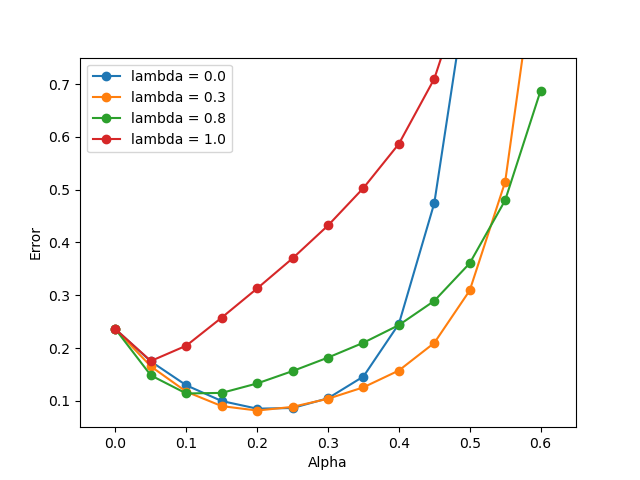
\includegraphics[width=0.8\linewidth]{figure4.png} 
    \caption{Average errors on the random-walk with single presentation for $\lambda = 0, 0.3, 0.8, 1$.}
    \label{fig:avg_errors_single_presentation}
\end{figure}


Various combinations of $\lambda$ and $\alpha$ were tested to analyze how different learning rates impact the learning outcomes.

The reproduced figure 2 illustrates the average error between the learned weights $w$ and the ideal weights $[\frac{1}{6}, \frac{1}{3}, \frac{1}{2}, \frac{2}{3}, \frac{5}{6}]^T$ for different values of $\lambda$ and $\alpha$. Each line in the figure represents the mean error for a specific value of $\lambda$ across different learning rates $\alpha$. The learning rate significantly affects the performance of TD learning. Lower $\alpha$ values (approximately between 0.2 and 0.3) produced the lowest prediction errors, indicating that a well-balanced learning rate achieves both fast convergence and high-quality weight updates.

As before, TD(1) performed the worst regardless of the $\alpha$ value, demonstrating the limitations of the conventional Widrow-Hoff approach in the bounded random-walk problem. In contrast, TD with $\lambda < 1$ produced better predictions.

While the reproduced results closely align with figure 4 from Sutton's paper, some discrepancies in the points where the lines for $\lambda = 0$ and $\lambda = 0.8$ intersect may be due to the different randomly generated training sets used in our experiments.

\begin{figure}[ht]
    \centering
    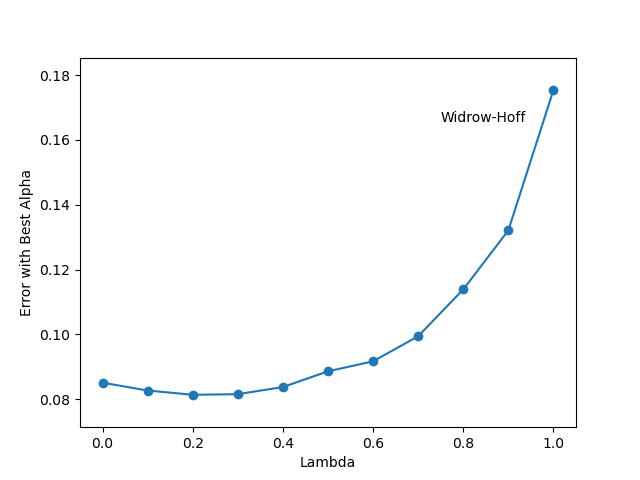
\includegraphics[width=0.8\linewidth]{figure5.png} 
    \caption{Average errors at best $\alpha$ on the random-walk problem with single presentation for $\lambda$.}
    \label{fig:avg_errors_best_alpha}
\end{figure}

The reproduced Fig. 3 illustrates the best mean errors for each $\lambda$ value, providing a more condensed view compared to Fig. 4. From the graph, it is evident that TD(1) produces the poorest predictions. The optimal $\lambda$ in the single presentation experiment is approximately 0.3. Similarly, the reproduced results closely align with those of the original Fig. 5.

\section{Results Analysis}

The analysis of our experimental results offers valuable insights into Temporal Difference (TD) learning, closely aligning with Sutton's foundational findings. In the repeated presentations paradigm, TD(1), similar to the Widrow-Hoff method, showed higher error rates compared to other $\lambda$ values, consistent with Sutton's observations. This indicates that our setup effectively captures the essential dynamics of TD learning.

In the single presentation paradigm, TD(0) outperformed other methods, reflecting its reliance on recent states and its congruence with maximum likelihood estimation in Markov processes. This further confirms the robustness of TD learning across different conditions.

Minor deviations were observed, such as slightly lower error rates in our experiments, likely due to stochastic training set generation and variability in initial weights and learning rate ($\alpha$ = 0.01). These factors may have contributed to the faster convergence and improved performance seen in our setup. Discrepancies in the intersection points of $\lambda = 0$ and $\lambda = 0.8$ in our reproduced Figure 4 highlight the subtle impact of initial conditions and dataset specifics on TD learning outcomes.

These variations underscore the sensitivity of TD learning to environmental factors and parameter choices, particularly the choice of $\lambda$. The observed differences in error rates suggest that contemporary computational practices or refinements might enhance TD learning performance. Moreover, the sensitivity of TD learning to $\lambda$ values emphasizes the need for careful consideration of this parameter to optimize predictive accuracy.

\section{Conclusion}

This report details the setup and implementation of the bounded random-walk process. Section II covers the generation of training sets, while Section III synthesizes the mathematical foundations from Sutton’s paper, explaining three learning paradigms: Supervised Learning (Widrow-Hoff), Incremental Learning TD(1), and the more general TD($\lambda$). Section IV presents the algorithms used to reproduce figures 3-5 in Sutton’s work, with a focus on two learning paradigms: repeated presentations and single presentation, along with their corresponding results and analysis.

The research process, encompassing paper review, code design, implementation, and result analysis, has provided a deeper understanding of Temporal Difference (TD) Learning, particularly regarding the impact of hyperparameters $\alpha$ and $\lambda$ on prediction outcomes. 

To ensure optimal results in future implementations of TD learning, careful evaluation of prediction problems (single-step vs. multi-step) is essential, alongside selecting an appropriate learning rate to balance convergence speed and accuracy. Finally, selecting the optimal $\lambda$ value based on problem specifics will leverage the strengths of TD learning, including incremental updates and improved predictive accuracy.


% \bibliographystyle{plainnat}
% \bibliographystyle{plain}
% \bibliography{references}

% \printbibliography
\bibliographystyle{unsrt}
\bibliography{references}

% \section*{Acknowledgments}
% This should be a simple paragraph before the References to thank those individuals and institutions who have supported your work on this article.



% {\appendix[Proof of the Zonklar Equations]
% Use $\backslash${\tt{appendix}} if you have a single appendix:
% Do not use $\backslash${\tt{section}} anymore after $\backslash${\tt{appendix}}, only $\backslash${\tt{section*}}.
% If you have multiple appendixes use $\backslash${\tt{appendices}} then use $\backslash${\tt{section}} to start each appendix.
% You must declare a $\backslash${\tt{section}} before using any $\backslash${\tt{subsection}} or using $\backslash${\tt{label}} ($\backslash${\tt{appendices}} by itself
%  starts a section numbered zero.)}



%{\appendices
%\section*{Proof of the First Zonklar Equation}
%Appendix one text goes here.
% You can choose not to have a title for an appendix if you want by leaving the argument blank
%\section*{Proof of the Second Zonklar Equation}
%Appendix two text goes here.}



% \section{References Section}
% You can use a bibliography generated by BibTeX as a .bbl file.
%  BibTeX documentation can be easily obtained at:
%  http://mirror.ctan.org/biblio/bibtex/contrib/doc/
%  The IEEEtran BibTeX style support page is:
%  http://www.michaelshell.org/tex/ieeetran/bibtex/
 
%  % argument is your BibTeX string definitions and bibliography database(s)
% %\bibliography{IEEEabrv,../bib/paper}
% %
% \section{Simple References}
% You can manually copy in the resultant .bbl file and set second argument of $\backslash${\tt{begin}} to the number of references
%  (used to reserve space for the reference number labels box).

% \begin{thebibliography}{1}
% \bibliographystyle{IEEEtran}

% \bibitem{ref1}
% {\it{Mathematics Into Type}}. American Mathematical Society. [Online]. Available: https://www.ams.org/arc/styleguide/mit-2.pdf

% \bibitem{ref2}
% T. W. Chaundy, P. R. Barrett and C. Batey, {\it{The Printing of Mathematics}}. London, U.K., Oxford Univ. Press, 1954.

% \bibitem{ref3}
% F. Mittelbach and M. Goossens, {\it{The \LaTeX Companion}}, 2nd ed. Boston, MA, USA: Pearson, 2004.

% \bibitem{ref4}
% G. Gr\"atzer, {\it{More Math Into LaTeX}}, New York, NY, USA: Springer, 2007.

% \bibitem{ref5}M. Letourneau and J. W. Sharp, {\it{AMS-StyleGuide-online.pdf,}} American Mathematical Society, Providence, RI, USA, [Online]. Available: http://www.ams.org/arc/styleguide/index.html

% \bibitem{ref6}
% H. Sira-Ramirez, ``On the sliding mode control of nonlinear systems,'' \textit{Syst. Control Lett.}, vol. 19, pp. 303--312, 1992.

% \bibitem{ref7}
% A. Levant, ``Exact differentiation of signals with unbounded higher derivatives,''  in \textit{Proc. 45th IEEE Conf. Decis.
% Control}, San Diego, CA, USA, 2006, pp. 5585--5590. DOI: 10.1109/CDC.2006.377165.

% \bibitem{ref8}
% M. Fliess, C. Join, and H. Sira-Ramirez, ``Non-linear estimation is easy,'' \textit{Int. J. Model., Ident. Control}, vol. 4, no. 1, pp. 12--27, 2008.

% \bibitem{ref9}
% R. Ortega, A. Astolfi, G. Bastin, and H. Rodriguez, ``Stabilization of food-chain systems using a port-controlled Hamiltonian description,'' in \textit{Proc. Amer. Control Conf.}, Chicago, IL, USA,
% 2000, pp. 2245--2249.



% \end{thebibliography}


% \newpage

% \section{Biography Section}
% If you have an EPS/PDF photo (graphicx package needed), extra braces are
%  needed around the contents of the optional argument to biography to prevent
%  the LaTeX parser from getting confused when it sees the complicated
%  $\backslash${\tt{includegraphics}} command within an optional argument. (You can create
%  your own custom macro containing the $\backslash${\tt{includegraphics}} command to make things
%  simpler here.)
 
% \vspace{11pt}

% \bf{If you include a photo:}\vspace{-33pt}
% \begin{IEEEbiography}[{\includegraphics[width=1in,height=1.25in,clip,keepaspectratio]{fig1}}]{Michael Shell}
% Use $\backslash${\tt{begin\{IEEEbiography\}}} and then for the 1st argument use $\backslash${\tt{includegraphics}} to declare and link the author photo.
% Use the author name as the 3rd argument followed by the biography text.
% \end{IEEEbiography}

% \vspace{11pt}

% \bf{If you will not include a photo:}\vspace{-33pt}
% \begin{IEEEbiographynophoto}{John Doe}
% Use $\backslash${\tt{begin\{IEEEbiographynophoto\}}} and the author name as the argument followed by the biography text.
% \end{IEEEbiographynophoto}




% \vfill

\end{document}


